%!TEX root = main.tex
\clearpage
\section{Conclusion}

\subsection{Global Vision}

In table \ref{tab:operators_status}, it's possible to understand the operators that was implemented in the first semestre of this dissertation. As can be seen, I have implemented \red{five} of thirteen operators that João Durães was especified.

In table \ref{tab:constraints_status}, is also possible to check that I have implemented \red{three} of eleven constraints related to the thirteen operators.

% \clearpage
\begin{table}[ht]
\begin{tabular}{c}
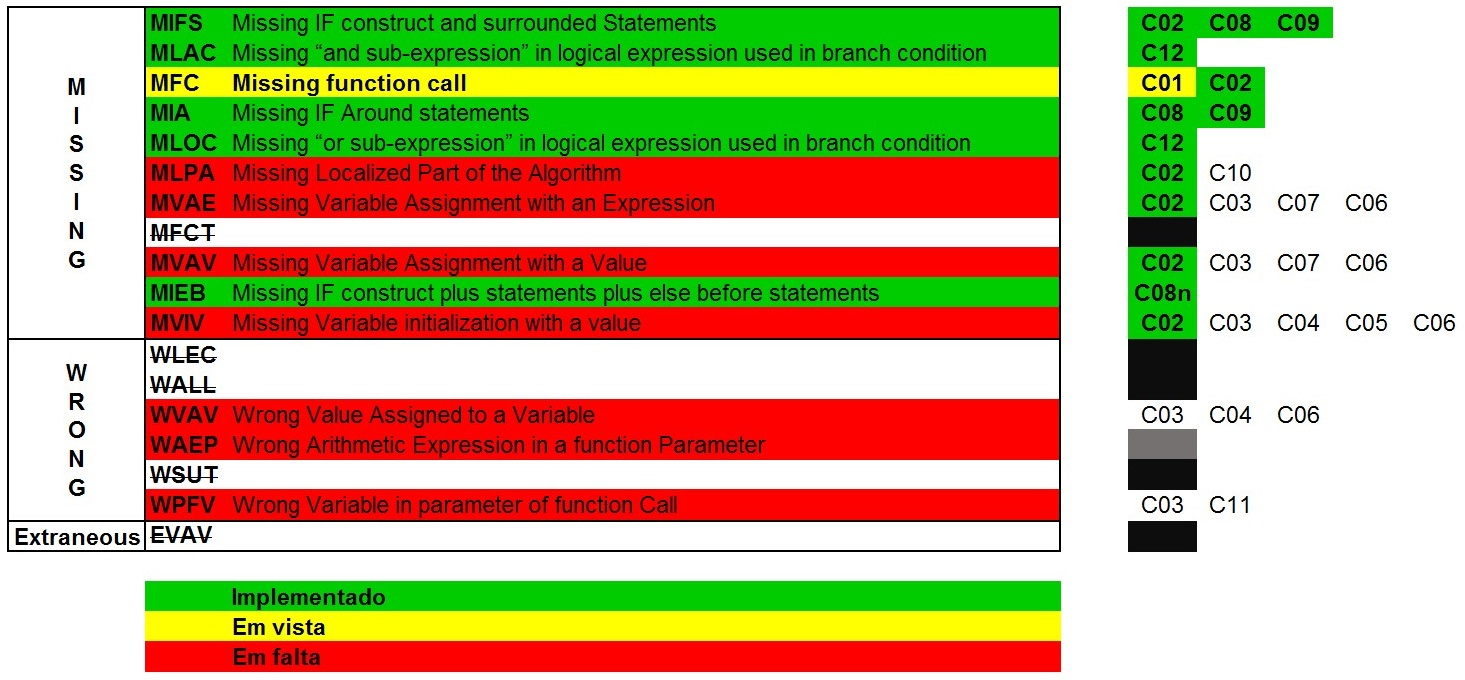
\includegraphics[width=1.1\textwidth]{img/operators_status.jpg}
\end{tabular}
\caption{\small \sl Operators Status and related constraints.\label{tab:operators_status}}
\end{table}



\begin{table}[ht]
\begin{tabular}{c}
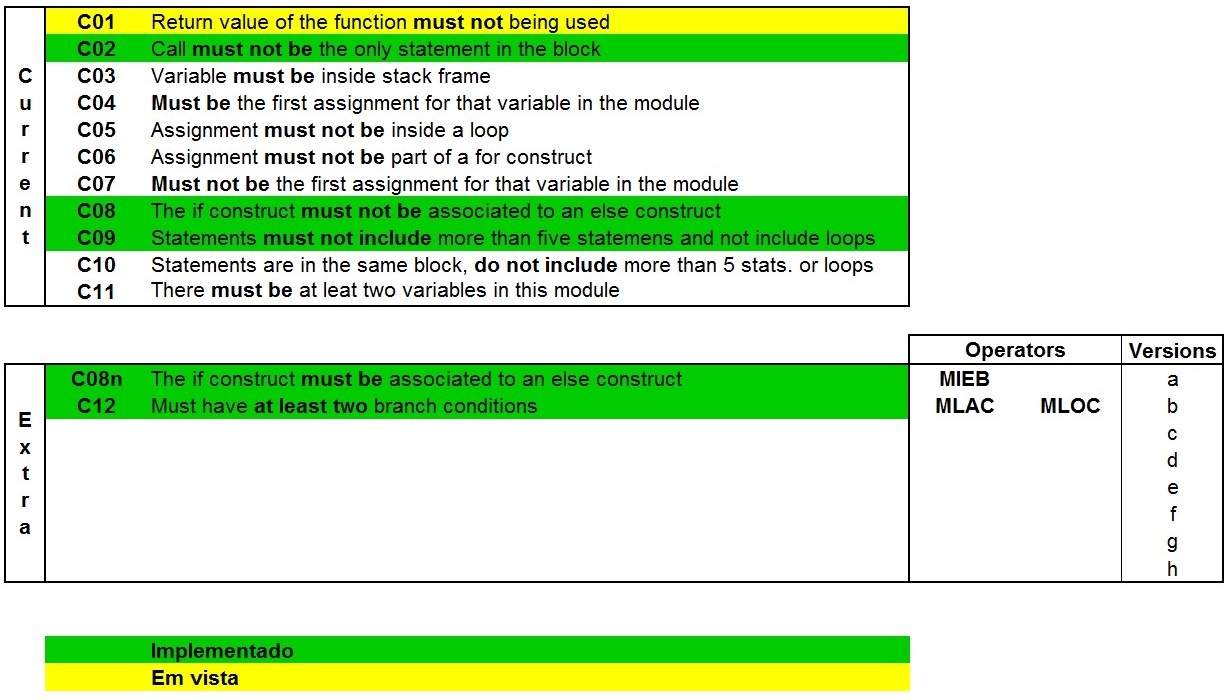
\includegraphics[width=1.1\textwidth]{img/constraints_status.jpg}
\end{tabular}
\caption{\small \sl Constraints Status.\label{tab:constraints_status}}
\end{table}

% \clearpage
\subsection{Future Work}

In the future, I have planned to implement the other operators and constraints. And apply this software in testing of open source softwares that I will select.

I will use \red{regression testing} to verify if when I coded one new operator or constraint I don't screwed the operators and constraints previous implemented.

\red{Regression Testing}

\red{System testing}

\red{Unit tests}